\documentclass[border=12pt]{standalone}
% shared preamble for all schematics/diagrams
\usepackage[siunitx, RPvoltages, european resistors]{circuitikz}
\usepackage{tikz}
\usetikzlibrary{arrows.meta,positioning,calc,shapes.geometric,fit,backgrounds,decorations.pathreplacing}
\usepackage[scaled=0.92]{helvet}
\renewcommand{\familydefault}{\sfdefault}
\usepackage{xcolor}
\usepackage{amsmath}
\usepackage{ifthen}
\definecolor{ink}{HTML}{1F2328}
\definecolor{muted}{HTML}{6B6A66}
\definecolor{c1}{HTML}{2A78D6}
\definecolor{c2}{HTML}{EB6834}
\definecolor{c3}{HTML}{1BAF7A}
\definecolor{c4}{HTML}{6250D6}
\definecolor{fill1}{HTML}{EAF2FC}
\definecolor{fill2}{HTML}{FDEEE7}
\definecolor{fill3}{HTML}{E6F6EF}
\definecolor{fill4}{HTML}{EFEDFB}
\definecolor{hv}{HTML}{C62828}
\ctikzset{bipoles/thickness=1.2, monopoles/ground/thickness=1.2}
\tikzset{every picture/.style={line width=0.7pt, color=ink}}

\begin{document}
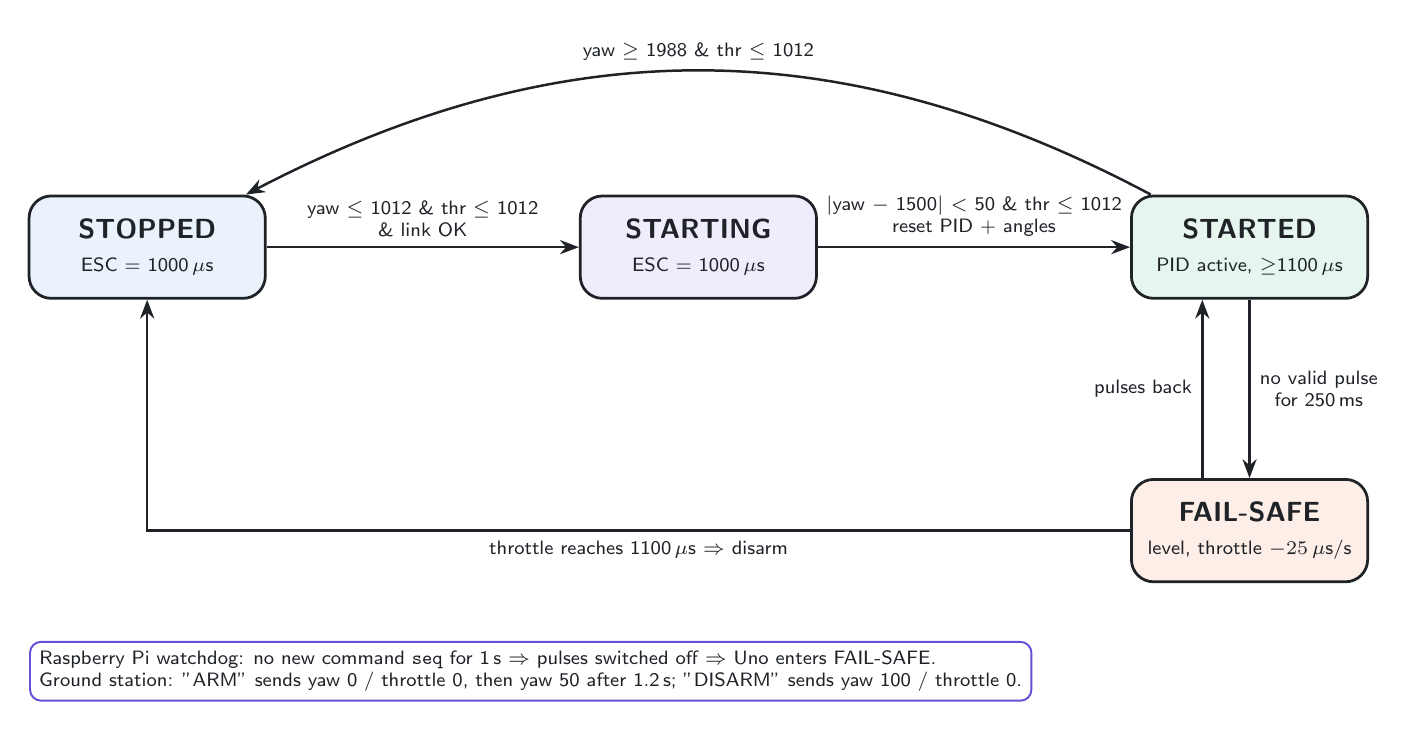
\begin{tikzpicture}[st/.style={draw, rounded corners=8pt, line width=1pt, minimum width=3cm, minimum height=1.3cm, align=center, fill=#1},
  a/.style={line width=0.9pt, -{Stealth[length=2.4mm]}}, l/.style={font=\scriptsize, align=center}]
\node[st=fill1] (s0) at (0,0) {\textbf{STOPPED}\\\scriptsize ESC = 1000\,$\mu$s};
\node[st=fill4] (s1) at (7,0) {\textbf{STARTING}\\\scriptsize ESC = 1000\,$\mu$s};
\node[st=fill3] (s2) at (14,0) {\textbf{STARTED}\\\scriptsize PID active, $\geq$1100\,$\mu$s};
\node[st=fill2] (fs) at (14,-3.6) {\textbf{FAIL-SAFE}\\\scriptsize level, throttle $-25\,\mu$s/s};
\draw[a] (s0) -- (s1) node[midway, above, l] {yaw $\leq$ 1012 \& thr $\leq$ 1012\\\& link OK};
\draw[a] (s1) -- (s2) node[midway, above, l] {$|$yaw $-$ 1500$|$ $<$ 50 \& thr $\leq$ 1012\\reset PID + angles};
\draw[a] (s2) to[bend right=28] node[midway, above, l] {yaw $\geq$ 1988 \& thr $\leq$ 1012} (s0);
\draw[a] (s2) -- (fs) node[midway, right, l] {no valid pulse\\for 250\,ms};
\draw[a] ([xshift=-6mm]fs.north) -- ([xshift=-6mm]s2.south) node[midway, left, l] {pulses back};
\draw[a] (fs) -| (s0) node[pos=0.25, below, l] {throttle reaches 1100\,$\mu$s $\Rightarrow$ disarm};
\node[draw=c4, fill=white, rounded corners, font=\scriptsize, align=left, anchor=north west] at (-1.5,-5.0) {
Raspberry Pi watchdog: no new command \texttt{seq} for 1\,s $\Rightarrow$ pulses switched off $\Rightarrow$ Uno enters FAIL-SAFE.\\
Ground station: "ARM" sends yaw 0 / throttle 0, then yaw 50 after 1.2\,s; "DISARM" sends yaw 100 / throttle 0.};
\end{tikzpicture}
\end{document}
